% This is a sample document using the University of Minnesota, Morris, Computer Science
% Senior Seminar modification of the ACM sig-alternate style. Much of this content is taken
% directly from the ACM sample document illustrating the use of the sig-alternate class. Certain
% parts that we never use have been removed to simplify the example, and a few additional
% components have been added.

% See https://github.com/UMM-CSci/Senior_seminar_templates for more info and to make
% suggestions and corrections.

\documentclass{sig-alternate}
\usepackage{color}
\usepackage[colorinlistoftodos]{todonotes}
\usepackage{multirow}

%%%%% Uncomment the following line and comment out the previous one
%%%%% to remove all comments
%%%%% NOTE: comments still occupy a line even if invisible;
%%%%% Don't write them as a separate paragraph
%\newcommand{\mycomment}[1]{}

\begin{document}

% --- Author Metadata here ---
%%% REMEMBER TO CHANGE THE SEMESTER AND YEAR AS NEEDED
\conferenceinfo{UMM CSci Senior Seminar Conference, April 2017}{Morris, MN}

\title{Automating Algorithm Design through Genetic Programming Hyper-heuristics}

\numberofauthors{1}

\author{
% The command \alignauthor (no curly braces needed) should
% precede each author name, affiliation/snail-mail address and
% e-mail address. Additionally, tag each line of
% affiliation/address with \affaddr, and tag the
% e-mail address with \email.
\alignauthor
Elsa M. Browning\\
	\affaddr{Division of Science and Mathematics}\\
	\affaddr{University of Minnesota, Morris}\\
	\affaddr{Morris, Minnesota, USA 56267}\\
	\email{brow3924@morris.umn.edu}
}

\maketitle
\begin{abstract}
	Automating algorithm design is a current subject of research in several different fields. One field that has approached it is hyper-heuristic optimization. Hyper-heuristics are heuristic search methods which seek to automate the process of selecting, generating, or adapting several simpler heuristics in order to solve computational search problems. This process is usually done with machine learning techniques, but in this paper we will be focusing on a family of algorithms within evolutionary computation called genetic programming. Hyper-heuristics that use genetic programming are simply called ``genetic programming hyper-heuristics." We will focus on one genetic programming hyper-heuristic in particular called autoconstruction. 
\end{abstract}

\keywords{Evolutionary Computation, Genetic Programming, Hyper-heuristics, Autoconstruction}

\section{Introduction}
\label{sec:introduction}
Since at least the 1950s, engineers have been trying to automate the design of algorithms~\cite{pappa:2014}. When we say 'automate the design of algorithms' this means we have been trying to reduce the amount of work people put in to the design process and have been trying to increase the amount of work the computer puts in. Two major approaches to this problem are meta-learning, in the field of supervised machine learning, and hyper-heuristics, in the field of optimization~\cite{pappa:2014}. While machine learning is out of the scope of this paper, it plays an important role in tackling the task of automating algorithm design.

One approach to the problem of automating algorithm design would be the use of hyper-heuristics; these are heuristic search methods which seek to automate the process of selecting, generating, or adapting several simpler heuristics in order to solve computational search problems. A \textit{heuristic} is a function that ranks alternatives in a search algorithm at each branching step and uses that information to choose which branch to follow. The goal of a heuristic is to find a solution in a reasonable amount of time that is capable of solving the problem at hand.

Hyper-heuristics can be classified under the field of Evolutionary Computation (EC), which is a subfield of artificial intelligence. EC encompasses algorithms that use techniques based on biological evolution to solve problems. A family of algorithms within EC, called genetic programming, uses biological techniques to evolve programs which then solve problems. When designing hyper-heuristics, engineers can use a several different kinds of algorithms to automate the process of selecting, generating or adapting several simpler heuristics, but one type of algorithm often used in this process is genetic programming. There are many variants of genetic programming, and the variant used can affect the success of the hyper-heuristic.

Traditionally, genetic programming solutions to problems evolve, but almost everything else is specified by the system designer \cite{spector:2016}. In a newer technique, called autoconstruction, the variation methods are evolving as well. Autoconstruction can be briefly defined as one or more parents producing one or more children, where the parents and children are programs which serve as potential solutions to a set of computational search problems. So autoconstruction can actually be thought of as a hyper-heuristic technique that uses genetic programming to evolve its solutions (which are in the form of programs), also known as a genetic programming hyper-heuristic.

In Sections~\ref{sec:evocomp},~\ref{sec:GP},~and~\ref{sec:HH} we describe necessary background for understanding the rest of this paper. Next, we describe the history of automating algorithm design with a focus on hyper-heuristics optimization in Section~\ref{sec:history}. Then, in Section~\ref{sec:gpvariants}, we go over a few different genetic programming variants used in hyper-heuristics and the success of two in particular. Next, we will go over current research being done with stack-based genetic programming (one of the GP variants) in Section~\ref{sec:ac}; the stack-based programming language called Push is used in this example along with a technique for automating algorithm design called autoconstruction. Finally we will go over the results and some conclusions in Sections~\ref{sec:results}~and~\ref{sec:conclusion} respectively.

\section{Background}
\label{sec:background}
In this Section, we introduce the field of Evolutionary Computation and define terminology used throughout the rest of the paper. Next we go over genetic programming, which is a family of algorithms in Evolutionary Computation used for evolving programs. Finally, we define what a hyper-heuristic is and go over a brief history on the development of hyper-heuristics. 
\subsection{Evolutionary Computation}
\label{sec:evocomp}
Evolutionary Computation (EC) is a subfield of artificial intelligence that uses algorithms based on biological evolution to solve problems. Much of the terminology in EC is based on biology as well. We will describe the general process of an EC algorithm in the following paragraph and define much of the basic terminology throughout this description.

These algorithms start with a group, or \textit{population}, of potential solutions to a problem or set of problems. These potential solutions, or \textit{individuals}, are tested on the problem (or set of problems) to determine how \textit{fit}, or well suited, the individuals are to solving that problem. This process is referred to as a \textit{fitness test}. Next, the less fit individuals are removed from the population. Finally, mutation and/or sexual reproduction are applied to the remaining individuals and the results are a new population, or the next \textit{generation}, of potential solutions. A \textit{mutation} is an insertion, deletion, or small change in the code or of an individual. It can also be a few flipped bits in a vector of 1s and 0s (which is often the format for EC algorithm solutions). For our purposes, we will focus on the first definition. \textit{Sexual reproduction} is when two or more individuals are combined in some way to create a new individual. When these techniques are applied to potential solutions, the original individual would be referred to as the \textit{parent}, and the new individual would be referred to as a \textit{child}. Parents can have more than one child. Occasionally, depending on the EC algorithms used, entirely new individuals, usually consisting of entirely random code, are introduced into the next population as well. This process is repeated until the \textit{global optima}, the best solution (or solutions) possible, is found, or until the algorithm hits a stopping point. Sometimes an algorithm is not able to find a global optima due to the algorithm not being good enough, so all programs have a designated stopping point to prevent them from running forever. The stopping point can be things like a time limit or a limit on the number of generations that can be produced.

EC has many applications which have seen success in medicine, engineering, and chemistry to name a few. Part of the field's success comes from its versatility~--~the techniques based on biological evolution can be applied to just about anything. Some examples that use these techniques include genetic algorithms, which are commonly used to generate high-quality solutions to search and optimization problems, ant colony optimization, which can be reduced to finding good paths through graphs, and artificial immune systems, which are computationally intelligent, rule based machine learning systems. In this paper, we will be focusing on a family of algorithms within EC called genetic programing.

\subsection{Genetic Programming}
\label{sec:GP}
Most EC algorithms produce solutions in the form of a single answer or set of answers to a problem. In genetic programming (GP), our solutions are in the form of programs. These programs then solve a problem (or class of problems), adding a level of abstraction to the problem solving process. This also automates a large part of the algorithm design process by allowing an algorithm to evolve rather than designing and revising the algorithm by hand.

GP works by encoding programs into a set of genes. These \textit{genes} can be thought of as a reorganization of a program for the evolution process. We then modifying those genes, usually with a genetic algorithm, to evolve a program which will perform well on a predefined task. The methods used to encode the programs into \textit{artificial chromosomes}, a sort of structure that holds the genes, and to evaluate the fitness of a program remain active research areas. There are several different GP representations and variations, but we will go into more detail on these in Section~\ref{sec:gpvariants}.

\subsection{Hyper-heuristics}
\label{sec:HH}
To better understand hyper-heuristics, we find it helpful to first define heuristic, discuss its purpose, and to work up from there. A \textit{heuristic} is a function that ranks alternatives in a search algorithm at each branching step and uses that information to choose which branch to follow. It uses \textit{domain knowledge}, or knowledge about the problem, to find solutions more quickly. If we look at the knapsack problem\footnote{the knapsack problem: given a set of items, each with a weight and value, determine the number of items to include in a collection so that the total weight is less than or equal to a given limit and the total value is as large as possible.}, a heuristic might be, given list X, "take the highest value item out of list X and put it into the knapsack. If the knapsack will be overweight, take the next highest valued item instead, etc. Repeat this process until the knapsack is full." The heuristic uses the knowledge of total weight a knapsack can hold and value of the items to find a solution to this problem.

\textit{Metahueristics}, often confused with hyper-heuristics, do not require domain knowledge to solve a problem. Metaheuristics can be thought of as general heuristics because a single metaheuristic could be used on many different problems (such as the knapsack problem, scheduling problems, and more).~\cite{tauritz:tutorial}

\textit{Hyper-heuristics} are heuristic search methods which seek to automate the process of selecting, generating, or adapting several simpler heuristics in order to solve computational search problems. These work indirectly on the solution space and work directly on the space of metaheuristics to solve problems~\cite{tauritz:tutorial}. Hyper-heuristics use a two step process; the first step is to create a set of algorithmic primitives appropriate for tackling a specific problem class and the second step is searching that algorithmic primitive space~\cite{harris:2015}. Genetic programming is often used to accomplish this second step~--~these hyper-heuristics are often referred to as Genetic Programming Hyper-heuristics.

\subsection{History of Hyper-heuristics}
\label{sec:history}
Automating algorithm design has been investigated by several different areas for at least 60 years. In the 1950s, the term ``machine learning" was defined as ``computers programming themselves"~\cite{pappa:2014}. This definition has changed over time to focus more on the learning aspect, but machine learning is still used to tackle the problem of automating the design of algorithms. While it plays an important role in the history of attempting to automate algorithm design, machine learning is out of the scope of this paper so it will not be discussed further.

Focusing on the automation of heuristic methods, we can trace the beginnings of hyper-heuristics to the 1960s (however, the term `hyper-heuristic' was not coined until 2000). Early approaches to developing hyper-heuristics focused on automatically setting the parameters of evolutionary algorithms. A \textit{parameter} used to be thought of as things like mutation rates and crossover, however the definition has expanded to include evolutionary algorithm components like selection mechanisms, and mutation and crossover operators. Many researchers still question which parameters to tune when designing hyper-heuristic systems. Traditionally, parameters are tuned before the evolution starts and controlled during the evolution. There are, however, exceptions. The idea of \textit{self-adaption}, where an algorithm is able to evolve parameters while solving a given problem, emerged later (see Section~\ref{sec:ac} for an example of this kind of system).~\cite{pappa:2014}

Today there are two major types of hyper-heuristics: \textit{heuristic selection} and \textit{heuristic generation}; the first focuses on selecting the best algorithm from a set of existing heuristics while the latter focuses on generating a new heuristic from the components of existing heuristics~\cite{pappa:2014}. The \textit{components} can be anything from the code of a heuristic function; this means it could be \textit{instructions}, for example adding two numbers together or determining if two strings are identical, or \textit{literals}, such as strings, integers, booleans, etc. We will be focusing on an example of heuristic generation discussed in Section~\ref{sec:autodog}.

\section{Genetic Programming Variants}
\label{sec:gpvariants}
Genetic programming~(GP) is the second step often used in the hyper-heursitc process. However, there are many different \textit{genetic programming variants}, or variations on the setup of GP algorithms, does it matter which one engineers use in their hyper-heuristic? Harris et al.~\cite{harris:2015} answers this question; they perform an experiment with five different GP variants to see if the variant chosen affects the success of a hyper-heuristic. The variants tested are Tree-based GP, Linear GP, Cartesian GP, Grammatical Evolution, and Stack-based GP~--~we will discuss tree-based and stack-based briefly in Sections~\ref{sec:tgp}~and~\ref{sec:sgp}. All of the listed variants were tested on the Boolean Satisfiability Problem~(SAT)\footnote{Harris et al. actually use a subproblem of SAT called 3-SAT. More information about the problem can be found in~\cite{harris:2015}}; the SAT problem is known for its complexity and NP-completeness, which is why Harris et al. chose it. To be \textit{NP-complete} means there is no known polynomial solution, and it is believed that one does not exist. SAT is also useful because many other difficult problems can be reduced to it. We will discuss the details of tree-based and stack-based GP due to their relevance in Section~\ref{sec:ac} and then go over the experiment and results in Section~\ref{sec:gpresults}.

\subsection{Tree-based Genetic Programming}
\label{sec:tgp}
Tree-based genetic programming~(TGP) is a form of GP variant that uses tree-based structures to represent programs.
\todo[inline, color=yellow]{add more about structure/pros/maybe cons, or cut}
\subsection{Stack-based Genetic Programming}
\label{sec:sgp}
\begin{table}
	\centering
	\begin{tabular}{|r|c|c|c|c|c|c|c|}
		\hline
		Input & 2 & 5 & sub & 2 & mult & 1 & equal\\
		\hline
		\multirow{3}{*}{Stack} & & & & & & & \\
		&   & 5 &   & 2 &   & 1 & \\
		& 2 & 2 & 3 & 3 & 6 & 6 & false \\
		\hline
	\end{tabular}
	\caption{Each column shows an input element and the contents of the Stack after processing that input.}
	\label{tab:stacks}
\end{table}

Stack-based GP~(SGP) represents programs in the form of linear sequences designed to be simpler and more efficient than tree-based GP. SGP uses data-stacks to manage the input and output of operations. To explain data-stacks, it's helpful to look at an example. If we have the program $(5-2)*2=1)$, we would first put it into \textit{postfix} notation, which is where any arguments or parameters for a command are stated before that command: \texttt{2~5~sub~2~mult~1~equal}. Here, `sub' means subtract, `mult' means multiply, and `equal' means take two numbers and return \texttt{true} if they are equal and \texttt{false} if they are not.

In Table~\ref{tab:stacks}, this program is shown being input into a stack. When the stack encounters \textit{terminals}, such as strings, integers, booleans, etc., they are simply pushed onto the stack. When the stack encounters \textit{primitives}, they are executed by taking elements off of the stack and pushing their results back onto the stack. For instance, if we look at the first part of the program, \texttt{(2~5~sub)}, we would push the 2 and 5 (which are terminals) onto the stack and then execute the subtract (which is a primitive). The subtract is executed by popping the top integer off of the stack, which would be 5, and popping the second integer off of the stack, which would be 2, and subtracting the second integer from the first, which would be $5-2$. The numbers are popped off in this order due to the first-in-last-out nature of stacks. We would then push the result, 3, back onto the stack. If, say, our program had started with \texttt{2 sub} instead, we would push the 2 onto the stack, and skip the subtract because there would not be enough arguments to execute it. This means the next part of the program would push 2 onto the stack, and execute the \texttt{mult} leaving 4 in the place of the 6 in the table.

At the end of Table~\ref{tab:stacks}, we can see that \texttt{false} is left on the stack. Generally, the top item on the stack at the end of a program is the answer to a problem that the program is trying to solve. Some SGP languages have multiple data-stacks, where there is a stack for each \textit{data type}, which are things like strings, integers, booleans, etc. This means that there is an execution stack, where the program is input, and separate stacks that the data is pushed onto depending on its data type. To see an example of a SGP with multiple stacks, see Section~\ref{sec:push}.

SGP are useful for hyper-heuristics because of the ability to skip instructions. This means, for example, that if a terminal is deleted from a program during the evolution phase, the program can still execute. SGP are also useful because of a special instruction called ``\texttt{dup}," which allows the program to duplicate a terminal on the stack. The ability to duplicate data is useful, especially when using a first-in-last-out language where data can get lost in stacks.

\subsection{Results}
\label{sec:gpresults}
\begin{figure}
	\centering
	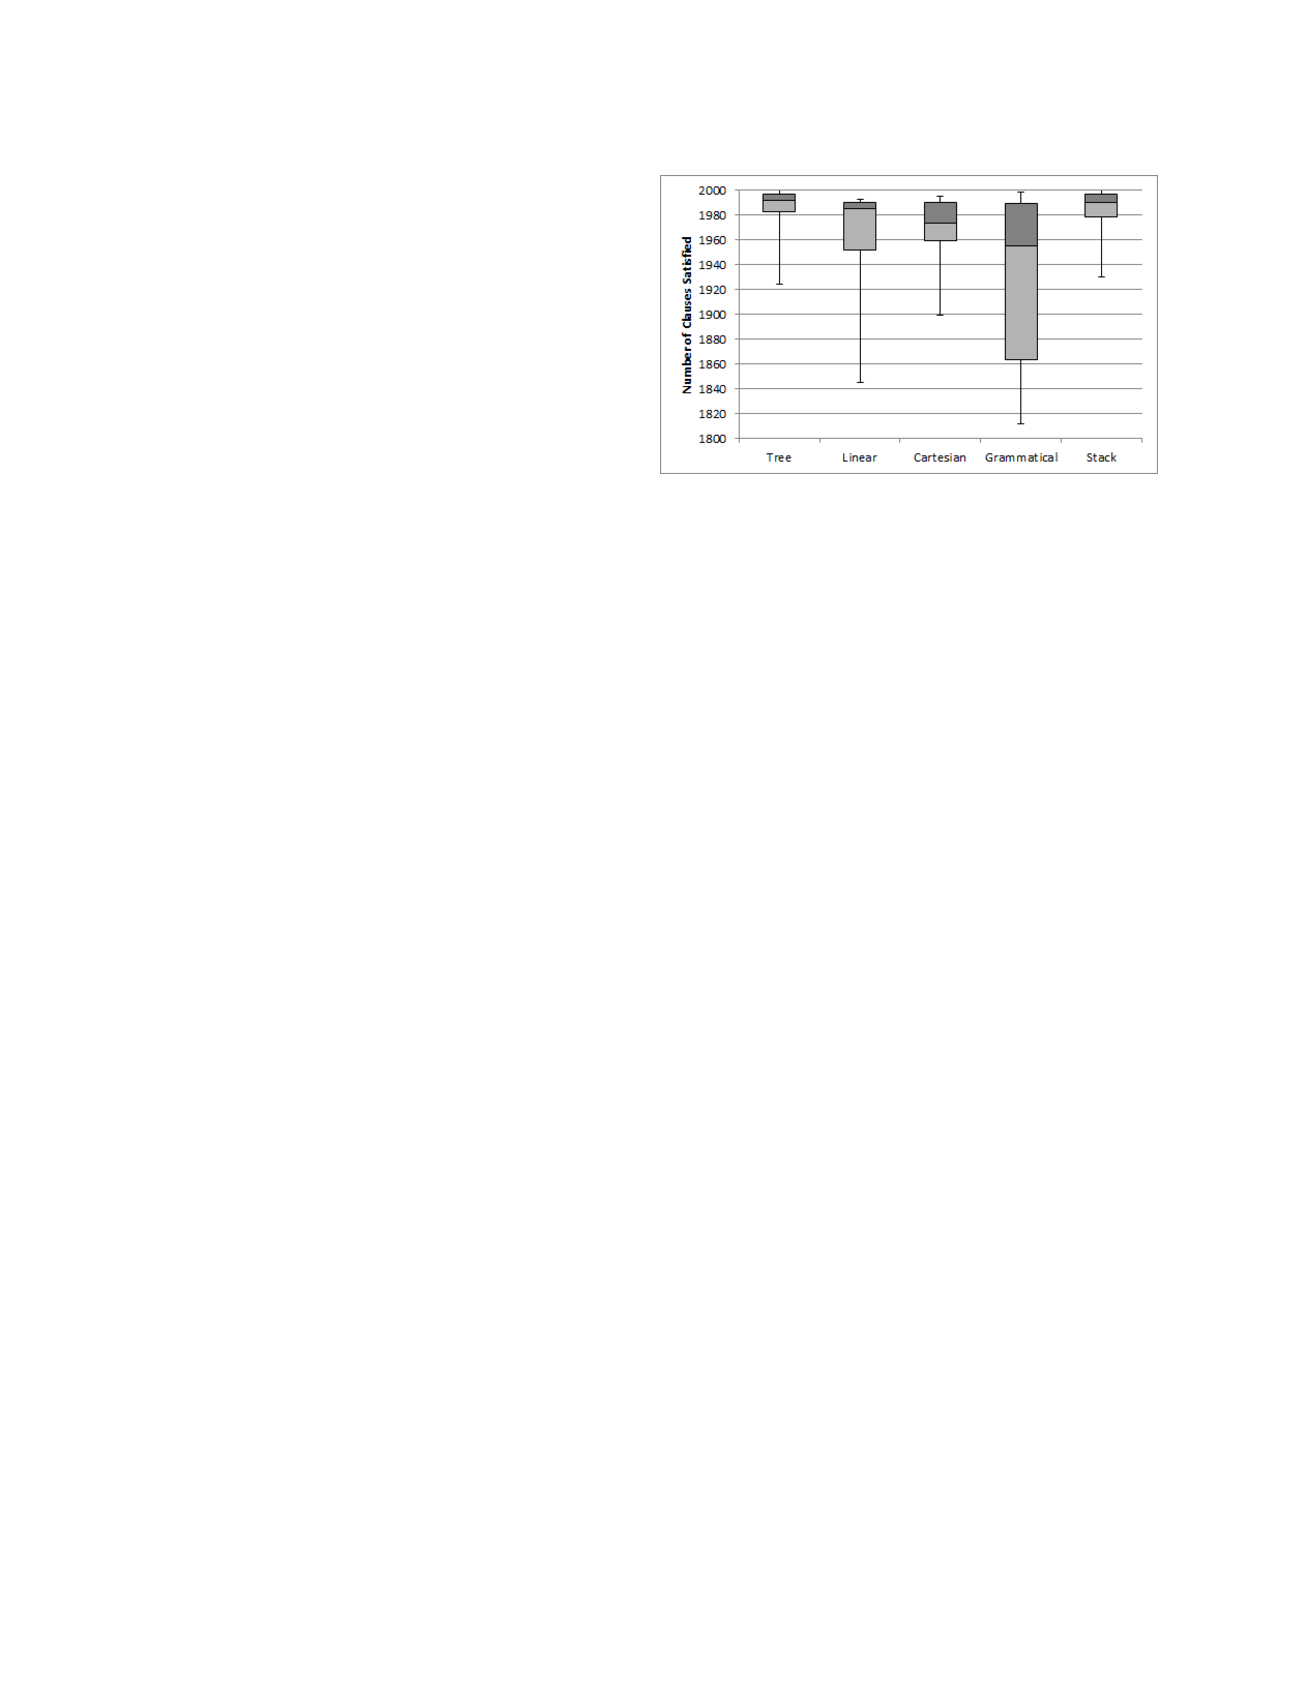
\psfig{file=gpvariant_graph.pdf,width =3.2in}
	\caption{Box plot showing the average number of SAT problem clauses that are satisfied by the best individuals from each run on the test set~\cite{harris:2015}.}
	\label{fig:gpvariants}
\end{figure}

To determine any differences in performance, the five GP variants were implemented in a common framework which facilitated sharing as much code as possible. This implementation may cause bias in the results, but this was a necessary risk because the alternative would cause similar bias; the alternative is attempting to maximize the performance of each GP variant at the cost of keeping a common implementation for all of the GP variants~\cite{harris:2015}.

The GP variants were tested on 2000 different instances, or \textit{clauses}, of the SAT problem. First each hyper-heuristic (which is the same except for the GP variant used) is run 30 times on a separate set of SAT clauses to "train" the hyper-heuristic. Next, the best individual program from each run of each hyper-heuristic is tested on the 2000 test clauses 3 separate times. These results are shown in Figure~\ref{fig:gpvariants}.

The results from Harris et al.~\cite{harris:2015} show that the GP variant chosen has a significant impact on the success of the hyper-heuristic. Tree-based GP and stack-based GP performed the best and performed similarly to one another. They solved more variations of the SAT problem on average than the other GP variants. Linear and Cartesian GP performed similarly to each other, but were not quite as good. Grammatical Evolution performed the worst. This does not mean that tree and stack are inherently better than other GP variants~--~it means that GP variants have different strengths and some are more suited to certain problem spaces than others. More testing is needed to find where each GP variant excels.

\section{Autoconstruction}
\label{sec:ac}
In genetic programming hyper-heuristics~(GPHH), the goal is to use genetic programming to evolve a program that will solve hard computational search problems. The individual programs serve as potential solutions. In most GPHH, the potential solutions are evolving, but everything else is specified by the system designer. \todo[inline]{not sure how to phrase previous sentence. Also not sure if I need to clarify what I mean by ``potential solutions"} In autoconstruction (a form of GPHH), evolution is evolving as well. This happens by encoding the methods of variation into the programs that are evolving so that, as a program evolves, its variation methods also evolve (see Section~\ref{sec:push} for how this works). 
\todo[inline, color=green]{TO NIC: is there more I could say to summarize autoconstruciton quickly or do you think this is fine? Should I say something about how autoconstruction = only genetic operator?}

Prior work on autoconstruction has explored a variety of system designs, but, until recently, none of them have been able to solve  problems. A new system called Autoconstructive Diversification of Genomes (AutoDoG) has broken this trend by solving at least one hard problem: Replace Space with Newline~\cite{spector:2016}. And, in recent unpublished work, AutoDoG has actually solved a problem called String Differences that has never been solved by other GP systems before~\cite{eva:2017}.
\todo[inline, color=yellow]{Not sure how much of this is introduction stuff}

\subsection{Push and Plush}
\label{sec:push}
Push is a stack-based programming language with a separate stack for each data type. It was developed for program evolution and autoconstruction was one of the driving forces behind the original design~\cite{spector:2016}. This is the programming language that AutoDoG, the system we describe in Section~\ref{sec:autodog}, uses. Push programs are strings of instructions, constants, and parentheses with only one syntax requirement: the parentheses must be balanced~\cite{lee:2001}. Instructions are executed by putting them on the \texttt{exec} stack. If the necessary arguments are not available for the instruction to be executed, the instruction is skipped. For example, assume all stacks are empty and assume a program says \texttt{(1 2 integer\_add)}. This means push 1 and 2 onto the \texttt{integer} stack and push the \texttt{integer\_add} onto the \texttt{exec} stack~\cite{lee:tutorial}. The \texttt{integer\_add} instruction will try to execute: the first two integers (in this case 1 and 2)  are popped off the top of the \texttt{integer} stack, added together, and the result (in this case 3) is pushed back on to the \texttt{integer} stack. Since there were enough arguments, the instruction executes: 1 and 2 are popped off the \textit{integer} stack and 3 is pushed onto the \textit{integer} stack. If, instead, the program was \texttt{(1 integer\_add)} then it would push 1 onto the \texttt{integer} stack, but skip the \texttt{integer\_add} because there are not enough integers in the \texttt{integer} stack for the instruction to execute. This would leave us with 1 on the \textit{integer} stack.

Plush is a linear genome format for Push~\cite{spector:2016}. This can be thought of as computerized DNA. It is a program in a linear format to make program evolution easier.
\todo[inline, color=green]{TO NIC: Is this accurate? This is how I have been thinking about linear genomes. Is this actually linear GP and using the registers (if so, should I talk about registers) or is it different?}
In Section~\ref{sec:autodog}, AutoDoG is actually evolving linear genomes and then translating those genomes back into Push programs~\cite{spector:2016}. This allows for methods of variation in a population to be encoded and evolved more easily. To aid in the translation process, Plush uses ``epigenetic close markers" (in other words, parenthesis) to separate blocks of code~\cite{spector:2016}. It also uses ``epigenetic silencing markers" to indicate when a part of the code in a genome should not be translated into a Push program~\cite{spector:2016}. This is arguably quite similar to how DNA and evolution work in biology in that some people are carriers for specific traits, but do not show them. This allows for these traits to be passed on to the next generation.
\todo[inline, color=green]{TO NIC: I might want to talk about why this is useful... why is this useful?}

\subsection{AutoDoG}
\begin{figure}
	\psfig{file=dlstandard.pdf,width =3in}
	\caption{explain graph~\cite{spector:2016}.}
	\label{fig:standard}
\end{figure}

\label{sec:autodog}
In this Section, we briefly describe some of the key features of AutoDoG.

When designing AutoDoG, Spector et al.~\cite{spector:2016} wanted to maintain diversity in parent selection. To do this, AutoDoG uses Lexicase Selection, described below: 

In each parent selection event,
\begin{itemize}
	\item start with a pool of the entire population
	\item filter the pool based on how each program performs on individual fitness cases (performed in random order, and one at a time)
	\item In each fitness case, only retain programs that are best on that case.
\end{itemize}
\todo[inline]{List or paragraph?}
\todo[inline]{Add more/better description of lexi (reread section in helmuth's dissertation)}

Its name comes from the way it filters the population using a kind of ``lexigraphic ordering" of cases \cite{spector:2016}. When tested on a benchmark suite of problems taken from introductory programming textbooks and compared to the results of other current GP parent selection techniques, Lexicase Selection allows for the solution of more problems in fewer generations~\cite{spector:2016}.
\todo[inline]{rephrase prev sentence?}

Another thing that Spector et al.~\cite{spector:2016} was concerned about when designing AutoDoG was cloning. This happens when an exact copy of a program moves on to the next generation. This is concerning because it can cause early convergence~--~it is possible that a population could lose all diversity and this could prevent the system from reaching a solution.
\todo[inline, color=green]{TO NIC: is this (prev sentence) actually a concern? I assume it is, but maybe it's so unlikely that it's not}
Cloning also significantly slows down the rate of evolution. This is bad because we want to reach a solution quickly. Most autoconstruction systems have some form of the ``no cloning rule," and AutoDoG has a form of this as well~\cite{spector:2016}. AutoDoG's version of this requires offspring to pass a more stringent diversification test in order to enter the population~\cite{spector:2016}. This test starts by taking an individual genome for the next generation. Then, that individual takes itself as a mate and makes temporary children. If the children differ enough from the individual and from each other, the individual enters the population and the children are discarded. If the individual fails, a random genome is generated and the test is repeated on the random genome. If the random genome fails, a blank genome (with no code in it) is generated and passed on to the next generation.

AutoDoG works similarly to PushGP, a reasonably standard generational programming system, but is run with autoconstruction as the sole genetic operator rather than using human designed mutation and crossover operators. In PushGP, the rate of mutation and crossover and other things is set by the designers. In AutoDoG, methods for making children are created by the designers, but the rates at which these methods are used or how the methods get used changes through the evolution of the program. For example, \texttt{genome\_uniform\_addition} is an instruction which inserts random instructions into a program with a likelihood taken from the top of the \texttt{:float} stack.
\todo[inline]{say more about this}

\subsection{Results}
\label{sec:results}
\begin{figure}
	\psfig{file=dlac.pdf,width =3in}
	\caption{explain graph~\cite{spector:2016}.}
	\label{fig:ac}
\end{figure}


AutoDoG is unique among autoconstructive systems in that it can solve hard problems. However, as stated by Spector et al.~\cite{spector:2016},
\begin{quotation}
	We do not know which of these, or which combinations of these, may be responsible for the fact that AutoDoG appears to be capable of solving more difficult problems than previous autoconstructive evolution systems.
\end{quotation}
This is because it's hard to separate the pieces; there are a lot of intertwined elements of AutoDoG and Push. Separating them to find exactly which elements contribute to the success without unraveling the entire system is difficult and has not yet been accomplished.
\todo[inline, color=green]{TO NIC: Is this (above) more correct?}

One challenging problem AutoDoG has solved is Replace Space with Newline (RSWN). This is a software synthesis problem that takes in a string and prints that string with all spaces replaced by newlines. It also must return the integer count of the non-whitespace characters. This is complex because it involves multiple data types, such as strings and integers, and multiple outputs.

AutoDoG does not actually do better than standard PushGP on this problem. It succeeds less reliably than PushGP. AutoDoG solves the RSWN problem 5--10\% of the time, producing general solutions~\cite{spector:2016}. This may not seem like much, but the fact that AutoDoG solves the problem at all is actually quite impressive. It is not surprising that AutoDoG performs less reliably because AutoDoG has to learn how to evolve as well as learn how to solve the problem. In recent unpublished work however, there may be examples of autoconstruction performing `better' than PushGP in a more meaningful sense; autoconstruction has found solutions to problems, such as String Differences, that have never been solved with regular PushGP (or any other GP system)~\cite{eva:2017}.

\todo[inline]{Add more info about new AutoDoG results}

One interesting thing to note about AutoDoG is how it evolves. In standard PushGP, one can see a steady incline in differences between the genomes of parents and their children. Over time, change occurs at a steady rate and is not very dramatic from one generation to the next. In AutoDoG, there are big differences between the genomes of some parents and their children. This is interesting because the methods for evolution are encoded into the genomes in AutoDoG. These DL graphs show us how evolution is affected from one generation to the next.


\todo[inline, color=yellow]{Clean up, more info about weird AutoDoG evolution.}
\section{Conclusions and Future Work}
\label{sec:conclusion}
Automating algorithm design has been undergoing research for at least the last 60 years. Hyper-heuristic optimization is a field that has devoted a lot of attention to this subject. Hyper-heuristics are heuristics that seek to automate the process of selecting, generating, or adapting simpler heuristics in order to solve computational search problems.
\todo[inline]{include more conclusion stuff to make up for stuff that was cut}
However, according to Pappa et al.~\cite{pappa:2014} in 2014, machine learning was ahead of hyper-heuristics optimization on the subject of automating algorithm design and ``can operate over different datasets, from different problem domains, and even with different features." This is not to say that hyper-heuristic optimization is no longer useful~--~using autoconstruction, a genetic programming hyper-heuristic for heuristic generation, engineers have had recent success solving the String Differences problem; this is exciting because it is a problem which has not been solved by a genetic programming system before~\cite{eva:2017}. has had recent success with solving String Differences. It would be interesting to see machine learning techniques combined with hyper-heuristics and is something that may happen in future work.

Something else that would be interesting to see is how different GP variants effect AutoDoG's success.
\todo[inline]{more summarizing and discussion}

\section*{Acknowledgments}
\label{sec:acknowledgments}


% The following two commands are all you need in the
% initial runs of your .tex file to
% produce the bibliography for the citations in your paper.
\bibliographystyle{abbrv}
% browning_paper.bib is the name of the BibTex file containing the
% bibliography entries. Note that you *don't* include the .bib ending here.
\bibliography{browning_paper}  
% You must have a proper ".bib" file
%  and remember to run:
% latex bibtex latex latex
% to resolve all references

\todo[inline, color=yellow]{Add last of references to bib}
\todo[inline, color=yellow]{note to self: all these notes take up about half a page!}

\end{document}


\subsection{My nifty subsection}
\label{sec:mysubsection}

I want to refer to Section~\ref{sec:evocomp}
and Figure~\ref{fig:twoColumnFigure}. It would also be nice
to cite~\cite{spector:2016} and~\cite{pappa:2014} and~\cite{eva:2017}.

Let's make an equation:
\[
\textrm{area} = \pi r^2
\]
I want to refer to Section~\ref{sec:typeChangesSpecialChars}
and Figure~\ref{fig:twoColumnFigure}. It would also be nice
to cite~\cite{spector:2016}.
We can also do inline equations: $s = \sum_{i=0}^N x_i$.
I want to refer to Section~\ref{sec:typeChangesSpecialChars}
and Figure~\ref{fig:twoColumnFigure}. It would also be nice
to cite~\cite{spector:2016}.\[
s = \sum_{i=0}^N x_i
\]

Typically, the body of a paper is organized
into a hierarchical structure, with numbered or unnumbered
headings for sections, subsections, sub-subsections, and even
smaller sections.  The command \texttt{\textbackslash section} that
precedes this paragraph is part of such a
hierarchy.\footnote{This is the second footnote.  It
	starts a series of three footnotes that add nothing
	informational, but just give an idea of how footnotes work
	and look. It is a wordy one, just so you see
	how a longish one plays out.} \LaTeX\ handles the numbering
and placement of these headings for you, when you use
the appropriate heading commands around the titles
of the headings.